\section{Implementation}\label{sec:03_impl}
% Explain section
This section explains the implementation based on the conceptual design introduced in \Sec{sec:02_design}. 
% MVC
As mentioned in PROBLM, the MVC architecture is used to implement this application.
% What is what
The models are introduced in \Sec{subsec:03_impl_models}, the views and controllers in \Sec{subsec:03_impl_servlets}.
% Others
Additionally, this implementation uses custom object stores (introduced in \Sec{subsec:03_impl_objstores}) and filters (introduced in \Sec{subsec:03_impl_filters}).


% !!!!
% MVC
% JAVA BEANS
% ...

% Object Store (User, Rooms, all Models + Beans)


\subsection{Models}\label{subsec:03_impl_models}
% Intro
As being mentioned, this project is implemented using the MVC pattern. Therefore, each entity of the chat system is represented by a model.
% Beans
Each model is implemented using the Java Bean specification. This enables to reuse models in \texttt{JSP} files.

% Figure
\begin{figure}[h]
\centering
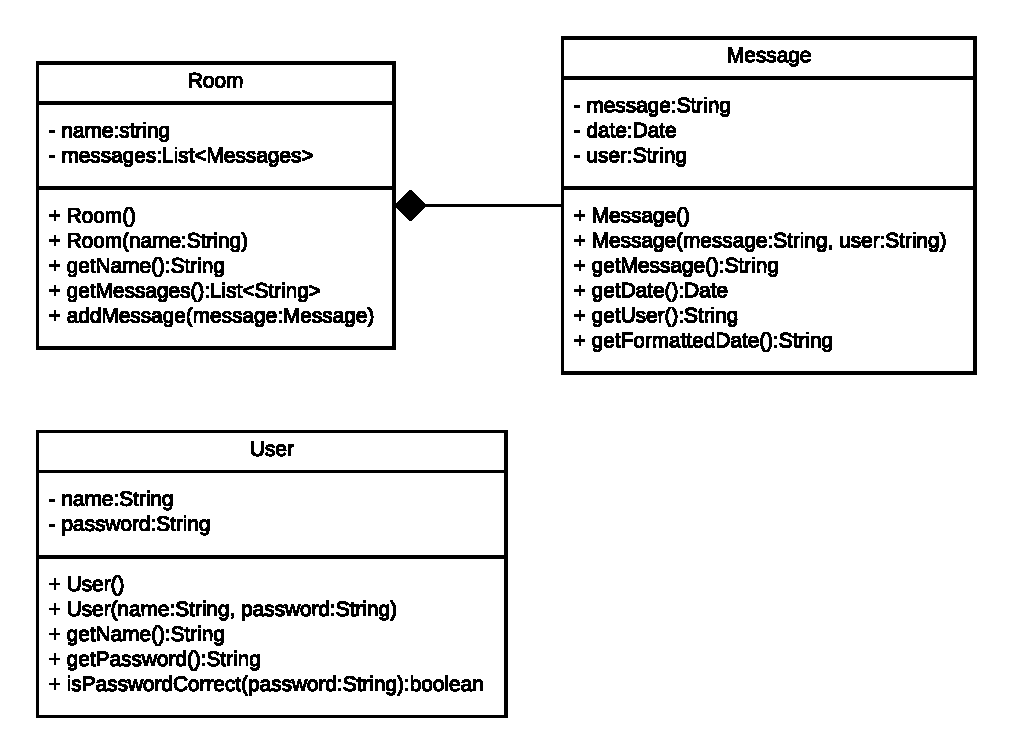
\includegraphics[scale=0.8]{images/03_impl/models}
\caption{Used models for the chat system}
\label{fig:03_impl_models_models}
\end{figure}

% Explain Figure
\Fig{fig:03_impl_models_models} shows all models used in the implementation of the chat system.
% Room and message
A \texttt{Room} models exists, which represents a room where users can chat with each other. Therefore, multiple messages are saved in a \texttt{Room}. A \texttt{Message} model represents a message send by any user in a specific room. Each \texttt{Message} is identified by its message-text, the name of the user, and the date when it was send.
% User
Each user is represented by a \texttt{User} model. This model is identified by the username, and the password.


% ==============
% ==============
\subsection{Object Stores}\label{subsec:03_impl_objstores}
% Why
As being mentioned in SEC DESIGN STORAGE, a custom store is needed to save the in \Sec{subsec:03_impl_models} introduced models.

Therefore, the following stores are being implemented:
\begin{itemize}
\item \texttt{UserStore}, saves \texttt{User} models
\item \texttt{RoomStore}, saves \texttt{Room} models
\end{itemize}
% Store functionality
Because a user and room can only exists once, a \texttt{Set}\footnote{Set (Java Platform SE 8) - \url{https://docs.oracle.com/javase/8/docs/api/java/util/Set.html}} data structure is used to save both Users, and Rooms. Furthermore, a store needs to provide the functionality to add an object to the store, get all objects from the store, or a specific one, and to check if an object has already been added to the store.


% Abstract class
Therefore, an abstract class called \texttt{ObjectsStore} is implemented, which implements the previously mentioned functionalities.
% Generics
The \texttt{ObjectStore} uses generics to implement the properties and methods. The \texttt{UserStore} and \texttt{RoomStore} implement this \texttt{ObjectStore} class and set the model (\texttt{User} and \texttt{Room}, respectively) for the generic type.
% Lifetime
The lifetime of an object saved to a store, is equal to the lifetime of the running webserver. As long as the webserver is running, an the objects are saved to memory.
% Lifetime of user
Except for the \texttt{UserStore}, which reads all \texttt{User} models from a text file, and write Users to a text file. Therefore, when the server restarts, all previously added \texttt{User} modes are available again.

%
% SINGLETON PATTERN !!!
%


% ==============
% ==============
\subsection{Servlets}\label{subsec:03_impl_servlets}
Fig XY shows the architecture of the in SEC DESIGN introduced routes. To implement this architecture, the following Servlets are implemented:
\begin{itemize}
\item \texttt{AuthLoginServlet}
\item \texttt{AuthLogoutServlet}
\item \texttt{LoginServlet}
\item \texttt{UserPageServlet}
\item \texttt{RoomServlet}
\item \texttt{RoomCreateServlet}
\item \texttt{AdminServlet}
\end{itemize}
% Views
Most of the mentioned servlets, own a specific view (a JSP file) which is saved in \path{Chat/src/main/webapp/views}.


\subsubsection{Authentication}\label{subsubsec:03_impl_servlets_auth}
For authentication, the AuthLoginServlet and the AuthLogoutServlet are created.
% Login
The \texttt{AuthLoginServlet} requires a \texttt{POST} request, and validates the request accordingly. If the given username and password are valid credentials (the user with the given name exist, and the password is correct), the \texttt{AuthLoginServlet} create a new \texttt{HTTPSession}, sets the active user, and the attribute \texttt{is\_authenticated} to \texttt{true}. This property is important for the \texttt{AuthFilter} introduced in SEC FILTER.]

% Logout
To logout, the AuthLogoutServlet exist. It invalidates the HTTPSession of an active user


\subsubsection{Login}\label{subsubsec:03_impl_servlets_login}
The LoginServlet shows a view called Login.jsp, which includes an HTML-form. The user has to insert the username and the password. Then the credentials are submitted to the AuthLoginServlet via a POST request.
If the credentials are parsed correctly by the AuthLoginServlet, the user is being redicrected to the user page, otherwise the servlet reloads itself.


\subsubsection{User}\label{subsubsec:03_impl_servlets_user}
The user servlet is responsible to list all available rooms. If the user clicks on a room link, the user will be redirected to the room.
% Empty rooms
If no rooms are available, the view shows a text and refers to the create-room page via a link. 

\subsubsection{Room}\label{subsubsec:03_impl_servlets_room}
When a user enters a room, the user can send messages. All user who are logged in and have entered the same room are able to see the messages. The room is saved as a attribute, called activeRoom, in the request. Therefore it is available as a Java Bean in the corresponding view. LST shows bla bla.

\subsubsection{Admin}\label{subsubsec:03_impl_servlets_admin}


% ==============
% ==============
\subsection{Filters}\label{subsec:03_impl_filters}

\subsubsection{Authentication}\label{subsubsec:03_impl_filters_auth}

\subsubsection{Admin}\label{subsubsec:03_impl_filters_admin}
